\documentclass[12pt]{article}
\usepackage[utf8]{inputenc}
\usepackage{amsmath}
\usepackage[T1]{fontenc}


\title{ECE 3413 Lab 04\\*Analysis of Linear Time Invariant (LTI) Systems}
\author{Leomar Dur\'an}
\date{${28}^{\text{th}}$ February 2023}

\usepackage{hyperref}

\usepackage[per-mode=symbol]{siunitx}
\newcommand*\siexpr[2][]{\SI[parse-numbers=false,#1]{#2}}%
\usepackage{xfrac}
\usepackage{amssymb}
\newcommand*\transpose{\mathsf{T}}

\usepackage{mathtools}%
\DeclarePairedDelimiter\brao()%
\DeclarePairedDelimiter\brac[]%
\DeclarePairedDelimiter\braco[)%
\DeclarePairedDelimiter\Brac\{\}%
\DeclarePairedDelimiter\norm\lVert\rVert%
\DeclarePairedDelimiter\piecefn\{.
\DeclarePairedDelimiter\evalat.|

\usepackage{lib/nonfloatenvirons}
\usepackage{booktabs}
\newcommand\ra[1]{\renewcommand*\arraystretch{#1}}
\ra{1.25}
\usepackage{minted}

\usepackage{adjustbox}
\newcommand*\mcadj[7]%
% {#columns}{col spec}{rotation}{adjust spec}
% {before rotated text}{rotated text}{after rotated text}
{%
    \multicolumn{#1}{#2}{%
        \rlap{%
            #5\adjustbox{rotate=#3,#4}{#6}~#7%
        }%
    }%
}

\usepackage{pdfpages}
\usepackage{standalone}
\usepackage{matlab}

\usepackage[skip=\baselineskip,indent=0pt]{parskip}
\setlength\parindent{0pt}

\def\hr{{\par\noindent\rule{\textwidth}{0.4pt}}}

\begin{document}

\maketitle
\newpage

\section{Introduction}

The purpose of this experiment is to apply the concept of transfer functions to a translational mechanical system.

The principles used in electrical engineering are shared with other disciplines of engineering.
We can apply these principles to help us look at everyday problems such as a translational system differently,
or we can use this familiarity to better understand the effect of a transfer function in a control system.

This lab also introduces a new type of transfer function, the state-space model which is represented by the \mintinline{matlab}{ss} class in Matlab.

\section{Procedure}

\subsection{Part 01}

\subsubsection{Step 01.01 -- The simulation}

\paragraph{The Parameters}

In part $1$ we are using standard input functions and applying the transfer function
$$
    G = \frac2{s^2 + 5 s + 9}
$$
to these.

I have written a Matlab script to parameterize the model so that it is more flexible and reusable.
This script is available in Appendix subsection \ref{sap:simulation params}.

It sets up the simulation time \mintinline{matlab}{TSTOP = 10.0} in \si\second, the parameters for the input function and the coefficients and constants for the transfer function.
In Part 01a, this input function is a step function which becomes \mintinline{matlab}{stepFinal = 1} in $\si\volt$ at time \mintinline{matlab}{Tstep = 0}.
In Part 01b, this input function is a ramp function $r(t)$ whose slope becomes $\SI1\volt$ at time \mintinline{matlab}{Tstep = 0} until $r(t) =$ \mintinline{matlab}{stepFinal = 1}.

This script is also reused in Part 02 since it already contains much of the input needed for part 02 (namely, the simulation time and transfer function.

\paragraph{01(a) The step response model}

In Part 01(a), we are modeling a step response. Thus, our input signal is a Heaviside step function as built in
the model on the following page.
% Fig. \ref{fig:step response model system}.
The only unique block in this model, the Step block is configured as in Fig. \ref{fig:step response model parameters}.

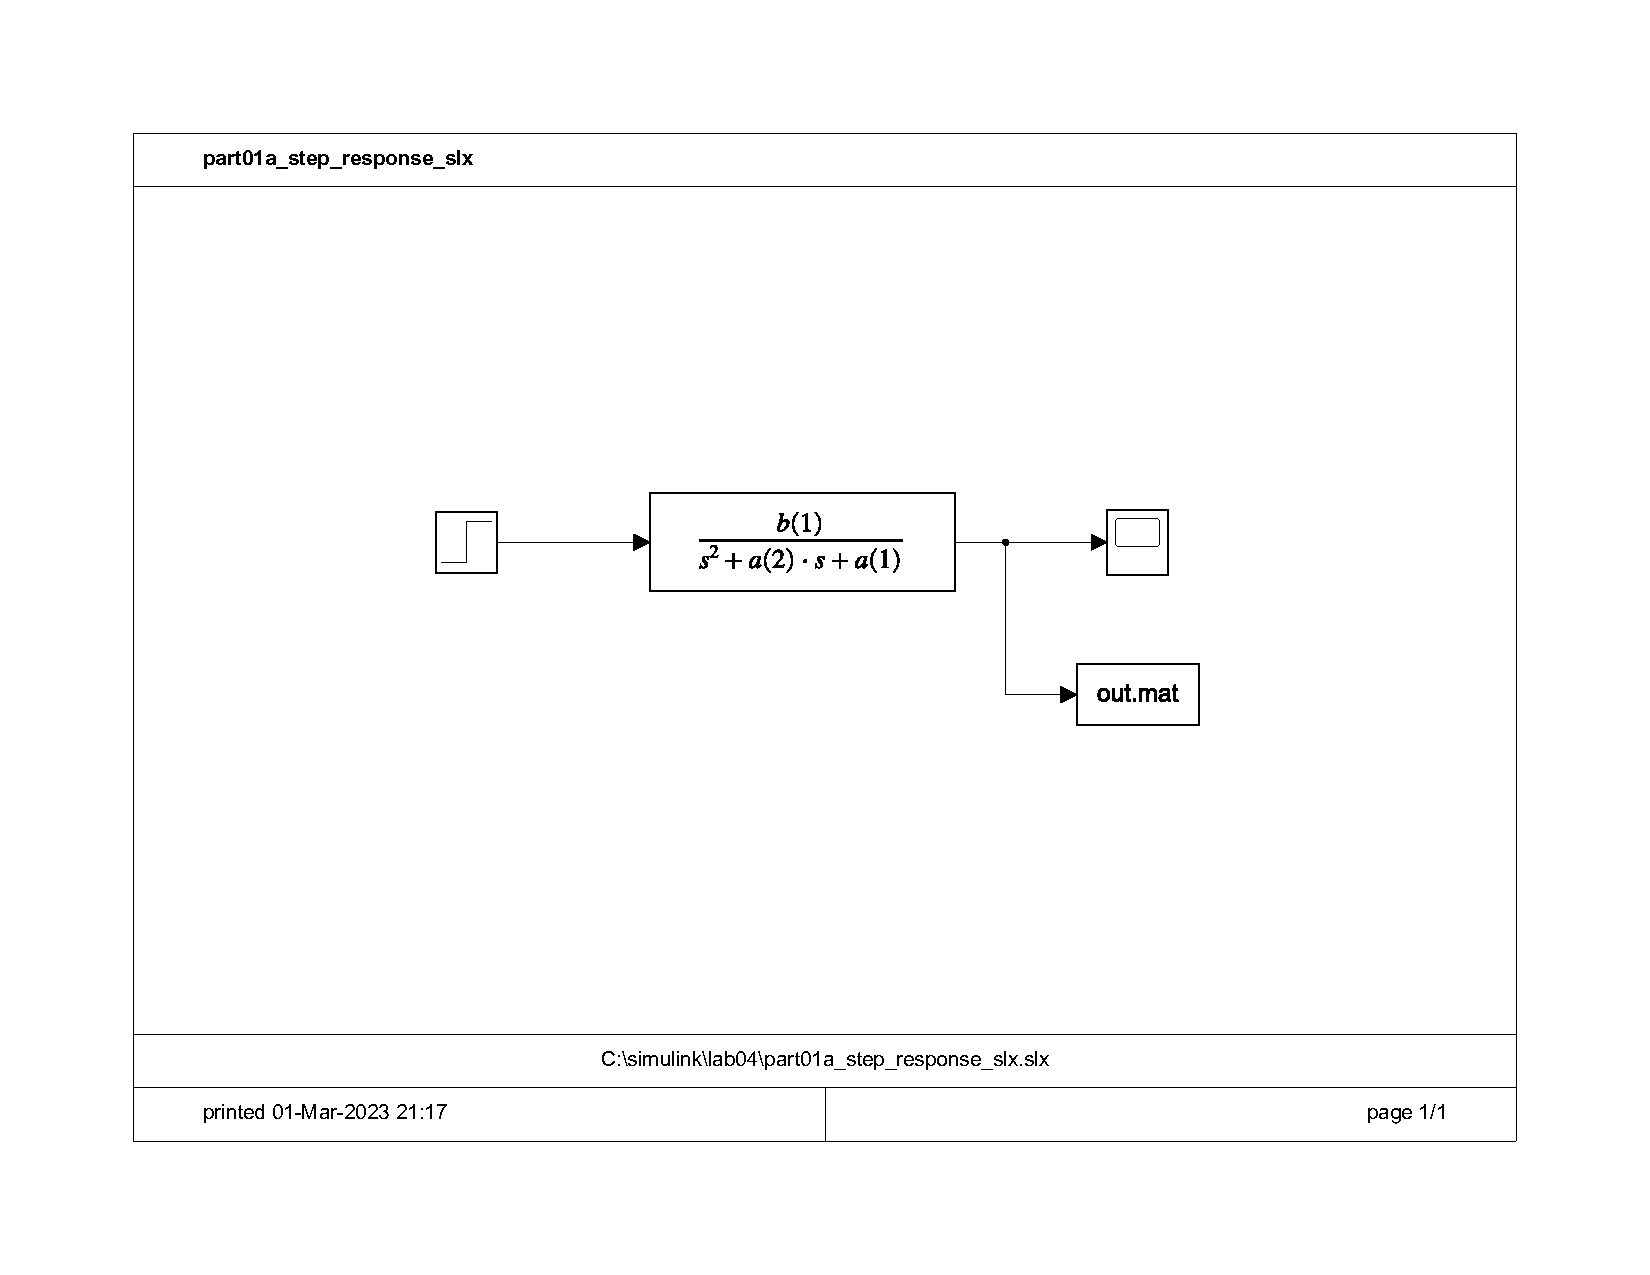
\includepdf[pages=1]{part01a_step_response_slx.pdf}

% \begin{figure}[h]
    % \centering
    % 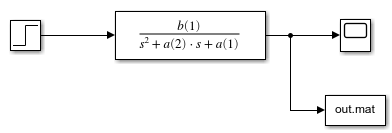
\includegraphics[width=\linewidth]{part01a_step_response_model.png}
    % \caption{The system over all for the step response.}
    % \label{fig:step response model system}
% \end{figure}

\begin{figure}[h]
    \centering
    % 689px = 5in
    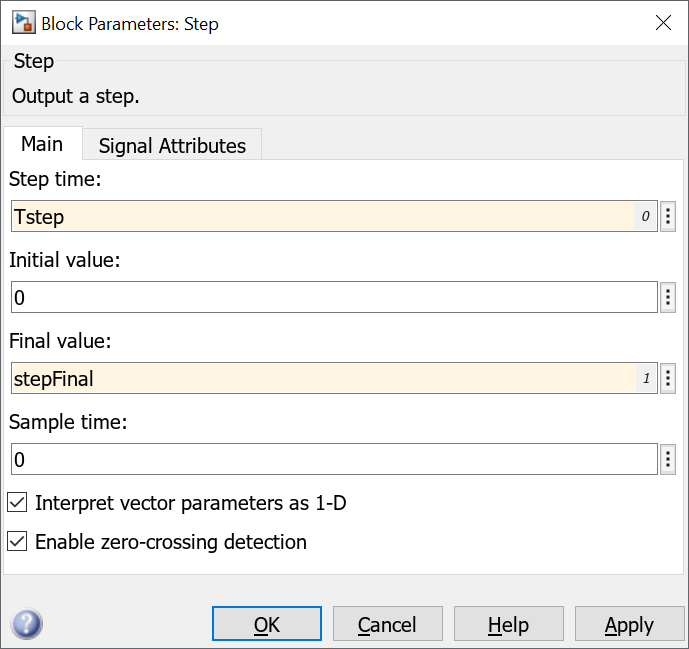
\includegraphics[width=(5in/689)*689]{part01a_step_parameters.png}
    \caption{The configuration for step.}
    \label{fig:step response model parameters}
\end{figure}

\paragraph{Common features}\label{par:common features}

The following features are common to all models simulated in this lab.
All parameters are defined in Appendix subsection \ref{sap:simulation params}.

\begin{figure}[h]
    \centering
    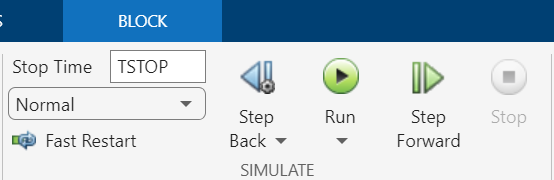
\includegraphics[width=(5in/689)*554]{common_simulation_time.png}
    \caption{The simulation time used in this equation is \mintinline{matlab}{TSTOP}.}
    \label{fig:common simulation time}
\end{figure}

\begin{figure}[h]
    \centering
    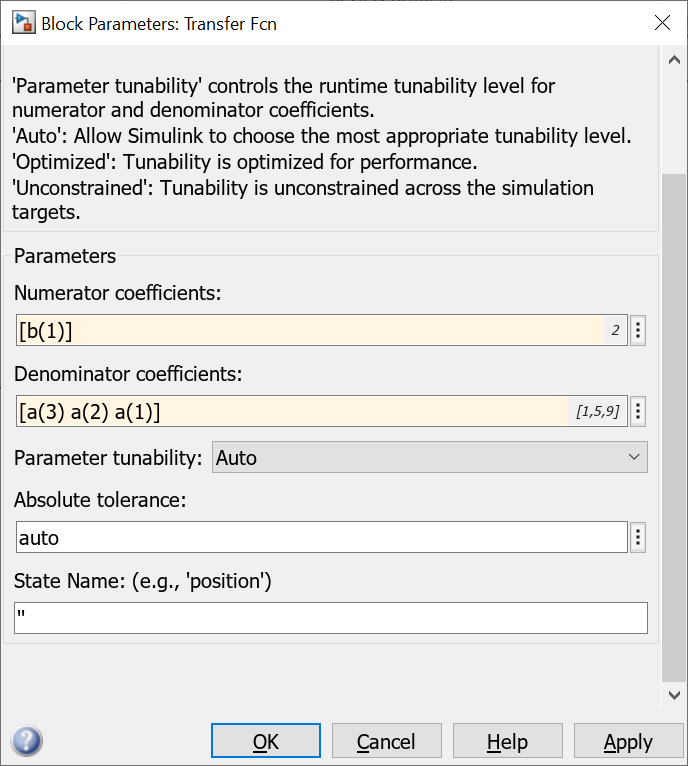
\includegraphics[width=(5in/689)*464]{common_transfer_fcn.png}
    \caption{The transfer function is $\frac{b_1}{s^2 + a_2 s + a_1}$. (Note that Matlab uses $1$-indexed arrays.)}
    \label{fig:common transfer fcn}
\end{figure}

\begin{figure}[h]
    \centering
    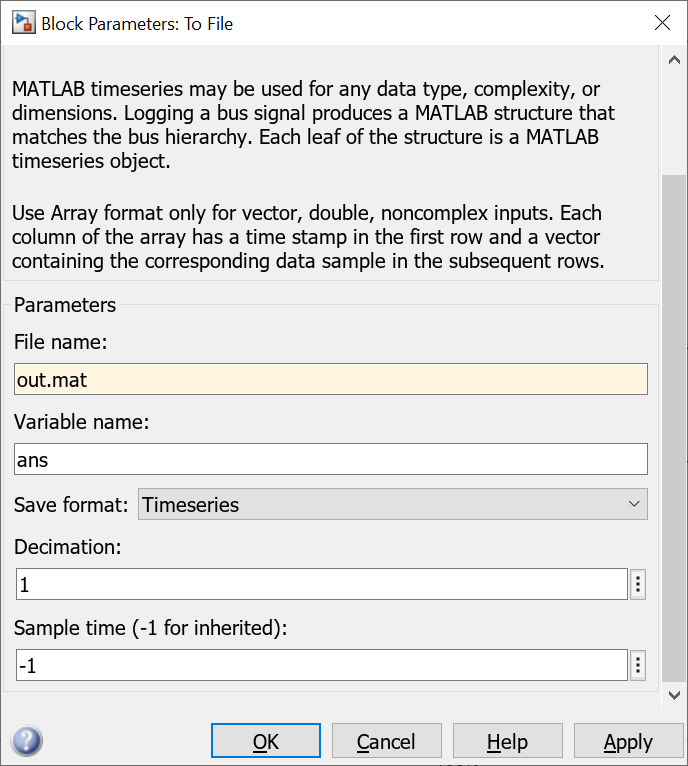
\includegraphics[width=(5in/689)*688]{common_to_file.png}
    \caption{All models will output the timeseries data of the response to the file \mintinline{matlab}{out.mat} to the default variable \mintinline{matlab}{ans}.}
    \label{fig:common to file}
\end{figure}

\paragraph{01(b) The ramp response model}

We use the same features described in paragraph \ref{par:common features}.
However, the difference is that we are modelling the ramp response seen
in the model on the next page.
% in Fig. \ref{fig:ramp response model system}
with the ramp parameters in \ref{fig:ramp response model parameters}.

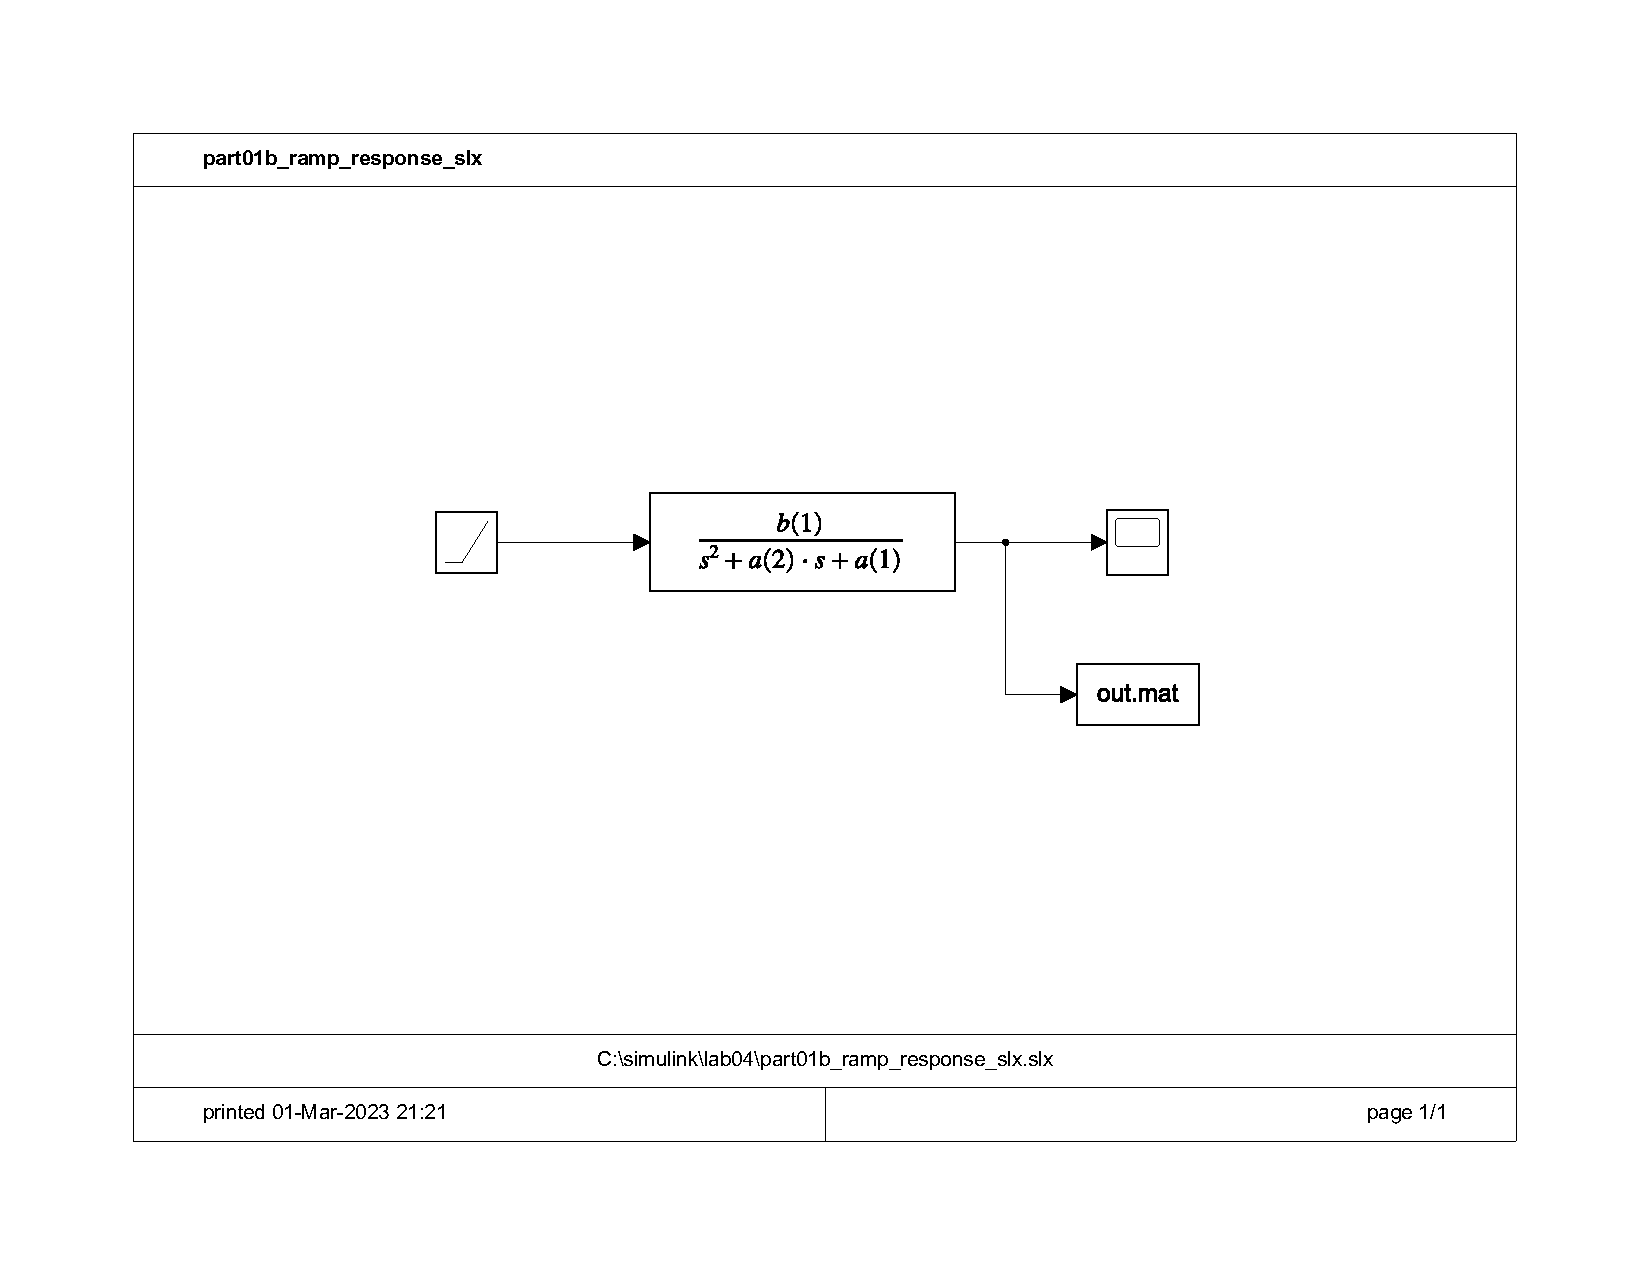
\includepdf[pages=1]{part01b_ramp_response_slx.pdf}

% \begin{figure}[h]
    % \centering
    % 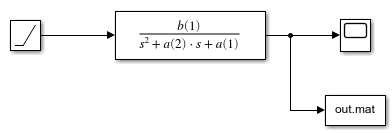
\includegraphics[width=\linewidth]{part01b_ramp_response_model.png}
    % \caption{The system over all for the ramp response.}
    % \label{fig:ramp response model system}
% \end{figure}

\begin{figure}[h]
    \centering
    % 689px = 5in
    %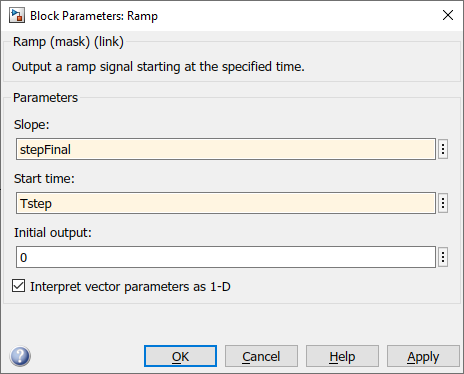
\includegraphics[width=(5in/689)*464]{part01b_ramp_parameters.png}
    \caption{The configuration for ramp.}
    \label{fig:ramp response model parameters}
\end{figure}

\subsubsection{Step 01.02 -- Measuring the traces on step response}

As before, we find the maximum

\paragraph{The peak} is found by finding the maximum output value of the plot.
We find the peak $c\brao{T_p} = \num{2.242e-1}$ in Fig. \ref{fig:step - measuring peak}.

\paragraph{The peak time} is the corresponding time, which we can find in the same plot.
The peak time $T_p \in \brac{{1.879}, {1.904}}\si\second$.
Let's take $T_p = \frac12\brao*{1.879 + 1.904}\si\second = \SI{1.8915}\second$.

\begin{figure}[h]
    \centering
    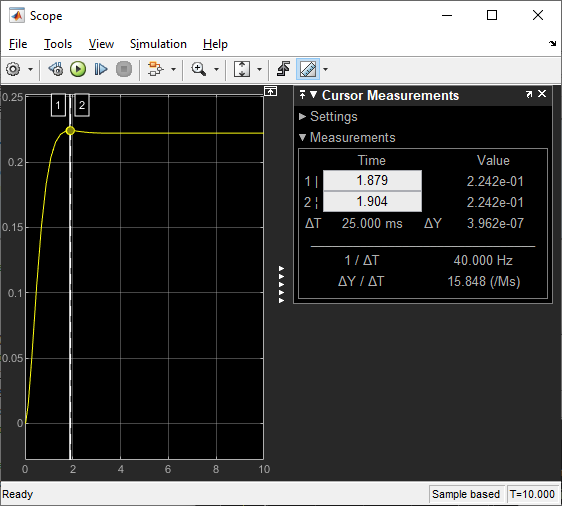
\includegraphics[width=\linewidth]{part01a_measuring_peak.png}
    \caption{Measuring the peak and peak time.}
    \label{fig:step - measuring peak}
\end{figure}

\paragraph{The percent overshoot} can be measured using Fig. \ref{fig:step - measuring percent overshoot}.
This is because cursor $1$ is at the peak time and cursor $2$ is on the final time.
So the percent overshoot is the value $\frac{\Delta Y}{c\brao{T_p}} = \frac{\num{1.929e-03}}{\num{2.242e-1}}\times\SI{100}\percent = \SI{0.8604}\percent$.
 
\begin{figure}[h]
    \centering
    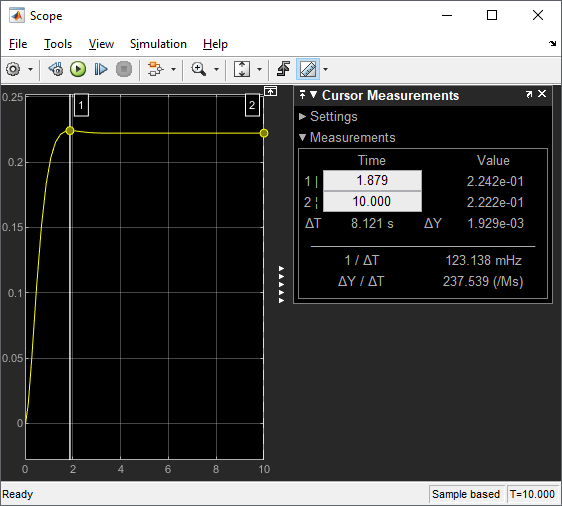
\includegraphics[width=\linewidth]{part01a_measuring_pcOS.png}
    \caption{Measuring the percent overshoot, final value and steady state error.}
    \label{fig:step - measuring percent overshoot}
\end{figure}

\paragraph{The stead state error}
We can also see the final value $c_f = \num{2.222e-1}$ in this figure,
and from that, we can calculate the steady state error.
We expect a final value equal to \mintinline{matlab}{stepFinal = 1}.
So $E_{ss} = 1 - \num{2.222e-1} = 0.7778$.

\paragraph{The rise time} To measure the rise time,
we must first find each of the first times when the output value is $\SI{10}\percent$ and $\SI{90}\percent$
of the final value.

\begin{figure}[h]
    \centering
    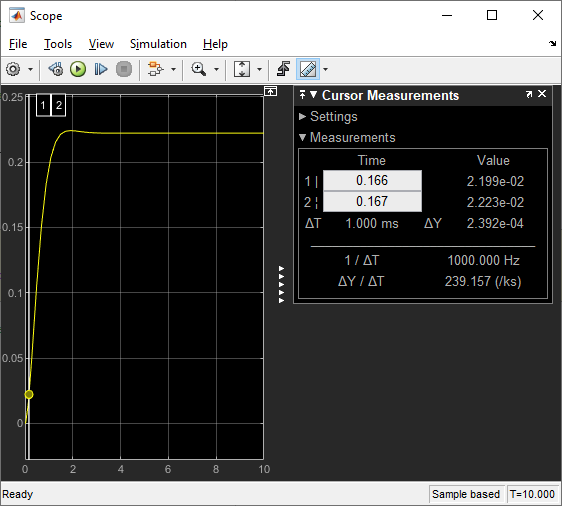
\includegraphics[width=\linewidth]{part01a_measuring_pc10.png}
    \caption{Estimating \SI{10}\percent of final output.}
    \label{fig:step - estimating 10 percent}
\end{figure}

Well, $\SI{10}\percent$ of the final value $\SI{10}\percent c_f = \SI{10}\percent \brao*{\num{2.222e-1}} = \num{2.222e-2}$.
In Fig. \ref{fig:step - estimating 10 percent}, we estimate the time when $c = \num{2.222e-2}$ to be
$$
	t_{.10} = \brao*{0.166 + \frac{\num{1e-3}}{\num{2.392e-02}}\brao*{\num{2.222e-2} - \num{2.199e-2}}}\si\second = \SI{0.16601}\second.
$$

\begin{figure}[h]
    \centering
    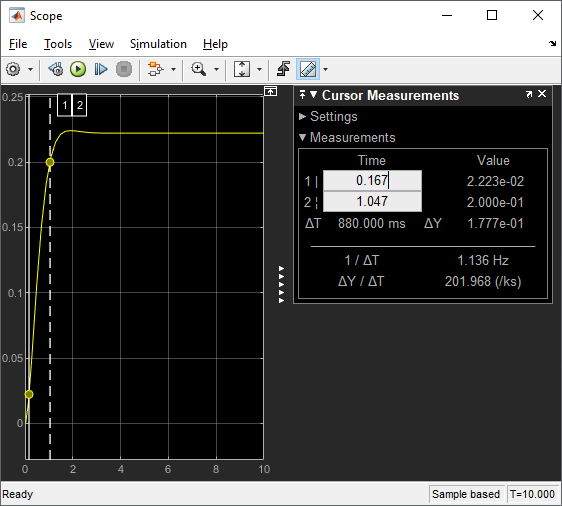
\includegraphics[width=\linewidth]{part01a_measuring_rise_time_estimate_+=.png}
    \caption{Measuring the rise time from $\SI{90}\percent$ and an estimate of $\SI{10}\percent$ of final output.}
    \label{fig:step - measuring rise time}
\end{figure}

Now $\SI{90}\percent$ of the final value $\SI{90}\percent c_f = 0.0200$.
In Fig. \ref{fig:step - measuring rise time}, we already have an exact measure of the time when $c = 0.0200$.
So let's just use that time $t_{.90} = 1.047$.
The time at cursor $1$ represents the closest time to $3$ decimal places.

The rise time $T_r = t_{.90} - t_{.10} = 1.047 - 0.16601 \si\second = \siexpr{0.88\overline099}\second$.

\paragraph{The settling time} is when the output reaches a value within $\SI5\percent$ of its final value.
Now, the signal can never supersede the maximum value of the signal, the peak $c\brao{T_p} = \num{2.242e-1}$.

However, $c_f + \SI{5}\percent = \num{2.222e-2}\brao{1 + .05} + \num{2.333e-2}$.
So we look for the last value where $c = c_f - \SI{5}\percent = \num{2.111e-2}$.
From Fig. \ref{fig:step - measuring setting time}, we see that this occurs at $T_s = \SI{1.208}\second$.

\begin{figure}[h]
    \centering
    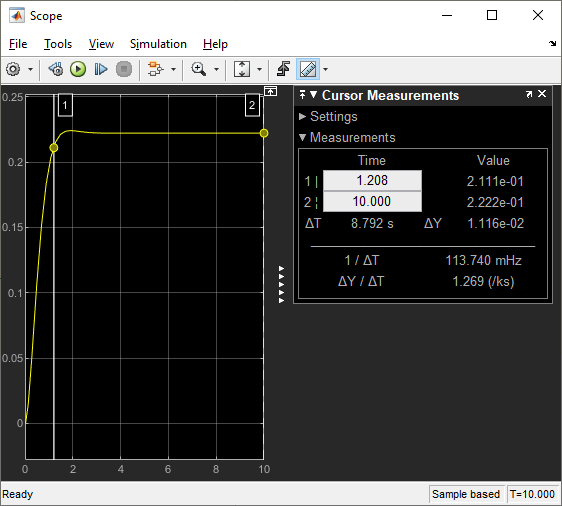
\includegraphics[width=\linewidth]{part01a_measuring_settling_time.png}
    \caption{Measuring the settling time.}
    \label{fig:step - measuring setting time}
\end{figure}

\subsubsection{Step 02 - Measuring the traces on ramp response}

% rise time
% 10%: 1.507
% 9.054 + 4.000e-3/8.889e-04 * (1.889e+0 - 1.8891)
% 9.049 + 5.000e-3/1.111e-03 * (1.8891 - 1.887e+0)
% 90%: 9.0585

% Peak, settling time
% 9.526 + 5.000e-3/1.111e-03 * (1.9941 - 1.993e+0)
% -5%: 9.5310

\paragraph{The peak} As before, we find the maximum output value of the plot.
We see in Fig. \ref{fig:ramp - measuring peak}, that the final value $\num{c_f = \num{2.099e+0}}$.

\paragraph{The peak time} The peak occurs at time $T_p = \SI{10.000}\second$.

\begin{figure}[h]
    \centering
    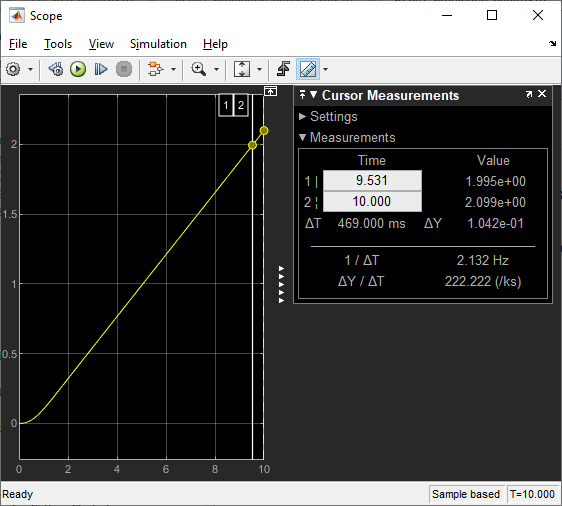
\includegraphics[width=\linewidth]{part01b_measuring_peak.png}
    \caption{Measuring the peak, peak time, the percent overshoot, final value, steady state error, and the settling time.}
    \label{fig:ramp - measuring peak}
\end{figure}

\paragraph{The percent overshoot}
In the case of the ramp response to the $G$, the maximum value is the final value.
Thus, the percent overshoot is $\frac{0}{2.099e+0} \times \SI{100}\percent = 0$.

\paragraph{The stead state error} is $1 - c_f = 1 - \num{2.099e+0} = -1.0990$.

\paragraph{The rise time} is the time it takes for the signal to rise
from $\SI{10}\percent$, $t_{.10} = \SI{1.507}\second$
to $\SI{90}\percent$, $t_{.90} = \SI{9.0585}\second$,
that is $T_r = \SI{9.0585}\second - \SI{1.507}\second = \SI{7.5515}\second.

\begin{figure}[h]
    \centering
    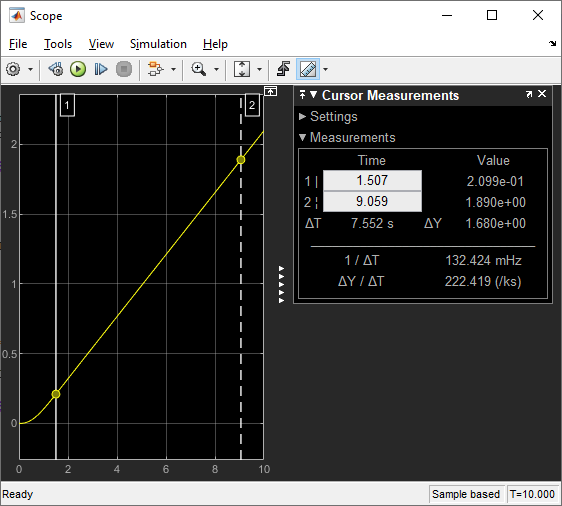
\includegraphics[width=\linewidth]{part01b_measuring_rise_time.png}
    \caption{Measuring the rise time from $\SI{90}\percent$ and an estimate of $\SI{10}\percent$ of final output.}
    \label{fig:ramp - measuring rise time}
\end{figure}

\paragraph{The settling time} can be see back in Fig. \ref{fig:ramp - measuring peak}.
The ramp response is within $\SI5\percent$ of the final value at time $T_s = \SI{9.5310}\second$.

\subsubsection{Step 01.03 -- Simulation analysis using Matlab}

To perform the analysis of the step and ramp response,
I have written the Matlab Live Script available in Appendix subsection \ref{sap:simulation analysis mlx}.

\subsection{Part 02 -- Writing in Matlab/Reading in Simulink}

We can write a signal in Matlab using a script such as that available in Appendix subsection \ref{sap:save sinusoid}
To analyze the effect of the transfer function on the generated sinusoidal function,
we use the model on the following page.

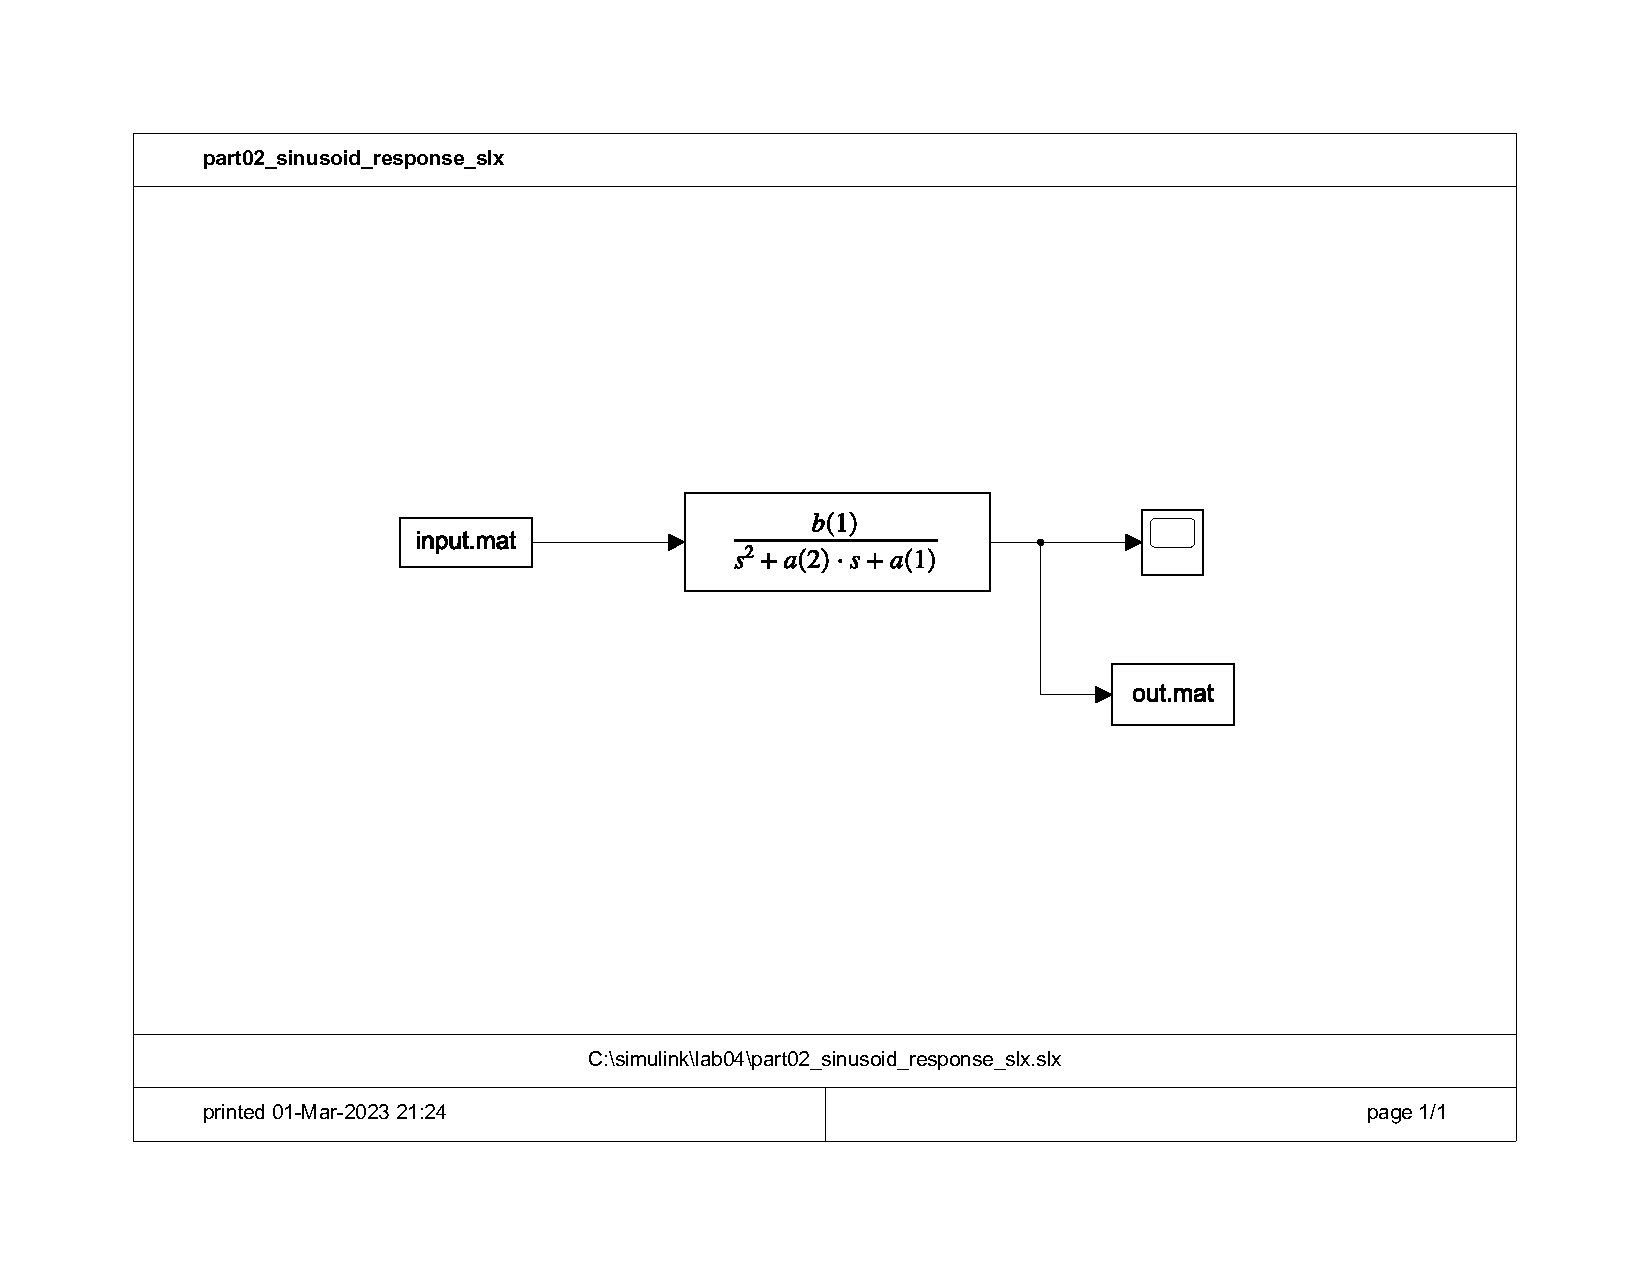
\includepdf[pages=1]{part02_sinusoid_response_slx.pdf}

\section{Results}

\hr

% This LaTeX was auto-generated from MATLAB code.
% To make changes, update the MATLAB code and export to LaTeX again.

\documentclass{article}

\usepackage[utf8]{inputenc}
\usepackage[T1]{fontenc}
\usepackage{lmodern}
\usepackage{graphicx}
\usepackage{color}
\usepackage{hyperref}
\usepackage{amsmath}
\usepackage{amsfonts}
\usepackage{epstopdf}
\usepackage[table]{xcolor}
\usepackage{matlab}

\sloppy
\epstopdfsetup{outdir=./}
\graphicspath{ {./part01_translational_mechanical_system_mlx_images/} }

\begin{document}

\matlabtitle{Part 1 $-$ Translational mechanical system}


\matlabheading{As a state-space model}

\begin{par}
\begin{flushleft}
is represented by the matrices of coefficients
\end{flushleft}
\end{par}

\begin{matlaboutput}
Mssr =
 
  A = 
       x1  x2  x3  x4  x5  x6
   x1   1   1  -1   0   0   0
   x2   1   0   0   0   0   0
   x3   1   0  -1  -1   0   1
   x4   0   0   1   0   0   0
   x5   0   0   0  -1   1   1
   x6   0   0   0   0   1   0
 
  B = 
       u1
   x1   1
   x2   0
   x3   0
   x4   0
   x5   0
   x6   0
 
  C = 
       x1  x2  x3  x4  x5  x6
   y1   0   0   0   0   0   1
 
  D = 
       u1
   y1   0
 
Continuous-time state-space model.
\end{matlaboutput}
\end{document}


\ \hr \\*

% This LaTeX was auto-generated from MATLAB code.
% To make changes, update the MATLAB code and export to LaTeX again.

\documentclass{article}

\usepackage[utf8]{inputenc}
\usepackage[T1]{fontenc}
\usepackage{lmodern}
\usepackage{graphicx}
\usepackage{color}
\usepackage{hyperref}
\usepackage{amsmath}
\usepackage{amsfonts}
\usepackage{epstopdf}
\usepackage[table]{xcolor}
\usepackage{matlab}

\sloppy
\epstopdfsetup{outdir=./}
\graphicspath{ {./part02_ratio_of_polynomials_form_mlx_images/} }

\begin{document}

\matlabtitle{Part 2 $-$ Rational of polynomials form}


\matlabheading{1. Conversion using Matlab}

\begin{par}
\begin{flushleft}
The transfer function from the state-space representation
\end{flushleft}
\end{par}

\begin{matlaboutput}
Mtf =
 
                   -s + 2.768e-16
  -------------------------------------------------
  s^6 - s^5 - s^4 - 2 s^3 + 2 s^2 + 2 s + 2.053e-16
 
Continuous-time transfer function.
\end{matlaboutput}

\matlabheading{2. Equation for transfer functions}

\begin{par}
\begin{flushleft}
create a transfer function that is just s
\end{flushleft}
\end{par}

\begin{matlaboutput}
T =
 
                   -s - 1.371e-16
  -------------------------------------------------
  s^6 - s^5 - s^4 - 2 s^3 + 2 s^2 + 2 s - 2.435e-16
 
Continuous-time transfer function.
\end{matlaboutput}

\matlabheading{Coefficient of determination $R^2$}

\begin{par}
\begin{flushleft}
To compare the transfer functions, let's find the $R^2$ value of all coefficients.
\end{flushleft}
\end{par}


\begin{par}
\begin{flushleft}
Then the R\textasciicircum{}2
\end{flushleft}
\end{par}

\begin{matlaboutput}
R2 = 1.0000
\end{matlaboutput}
\begin{matlaboutput}
shows that the coefficients have a strong correlation
\end{matlaboutput}
\begin{matlaboutput}
and are therefore equivalent.
\end{matlaboutput}
\end{document}


\section{Discussion}

After finding the state-space representation,
this experiment becomes very straightforward.
However, that is the difficult part.

What I remembered to help me finish it is that springs act on displacement into the moving mass and viscous dampers aft on velocity away from the moving mass.
After this, the sum of all forces must equal the acceleration of the mass.
Then setting up the matrix of coefficients is not difficult although I may not have been able to think of coming up with the variables myself.
It's a really clever way of solving this problem.

This experiment shows application not only in electrical engineering, but also mechanical and civil engineering of the concept of a control system.
It's interesting to imagine how many of the concepts that we have learned in electrical engineering may be applied to other engineering disciplines or may have even come from methods in other engineering disciplines.

Often times, it seems that less intuitive techniques may make a problem much easier to solve simply by changing the domain or a basis.
This is the principle behind using the Laplace transform to handle transfer functions more easily.

\newpage
\appendix
\section{Appendix}

\subsection{Step 01 (in parts 01 and 02) -- Simulation parameters, Matlab Script}\label{sap:simulation params}
\inputminted{matlab}{step01_simulation_params.m}

\hr

\subsection{Part 01 Step 03 -- Simulation analysis, Matlab Live Script}\label{sap:simulation analysis mlx}
\inputminted{matlab}{step03_simulation_analysis_mlx.m}

\hr

\subsection{Part 02 -- Saving a sinusoidal function}\label{sap:save sinusoid}
\inputminted{matlab}{part02_save_sinusoid.m}

\end{document}
